\etbox{h}{box:information}{The Pulse Tube cryocooler}
{The Pulse Tube cryocooler (PT) is based on the displacement and the expansion of a gas, usually He$^4$. The working fluid undergoes an oscillating flow and an oscillating pressure. A typical average pressure in a PT is $25}$ bar, and a typical pressure amplitude is $2$ � $7$ bar. \\
A piston compressor and a set of switching valves  are used to create the pressure oscillations of the helium gas.  A crucial element of the cryocooler is the  PT regenerator. It is a heat exchanger, which acts as �cold storage� systems for the  pulsed flow processes used in the cryocooler. \\
In fact, when the piston moves periodically pushing the gas, which enters the regenerator with temperature $T_h$ and leaves it  at the cold end with temperature $T_c$, hence heat is transferred into the regenerator material. On its return the heat stored within the regenerator is transferred back into the gas.\\
In practice, the regenerator  stores the energy from one stream and later transfer the energy to a second stream, for example between the out-of-phase pulses of gas. 
\FloatBarrier
\begin{figure}[H]
	\begin{center}
		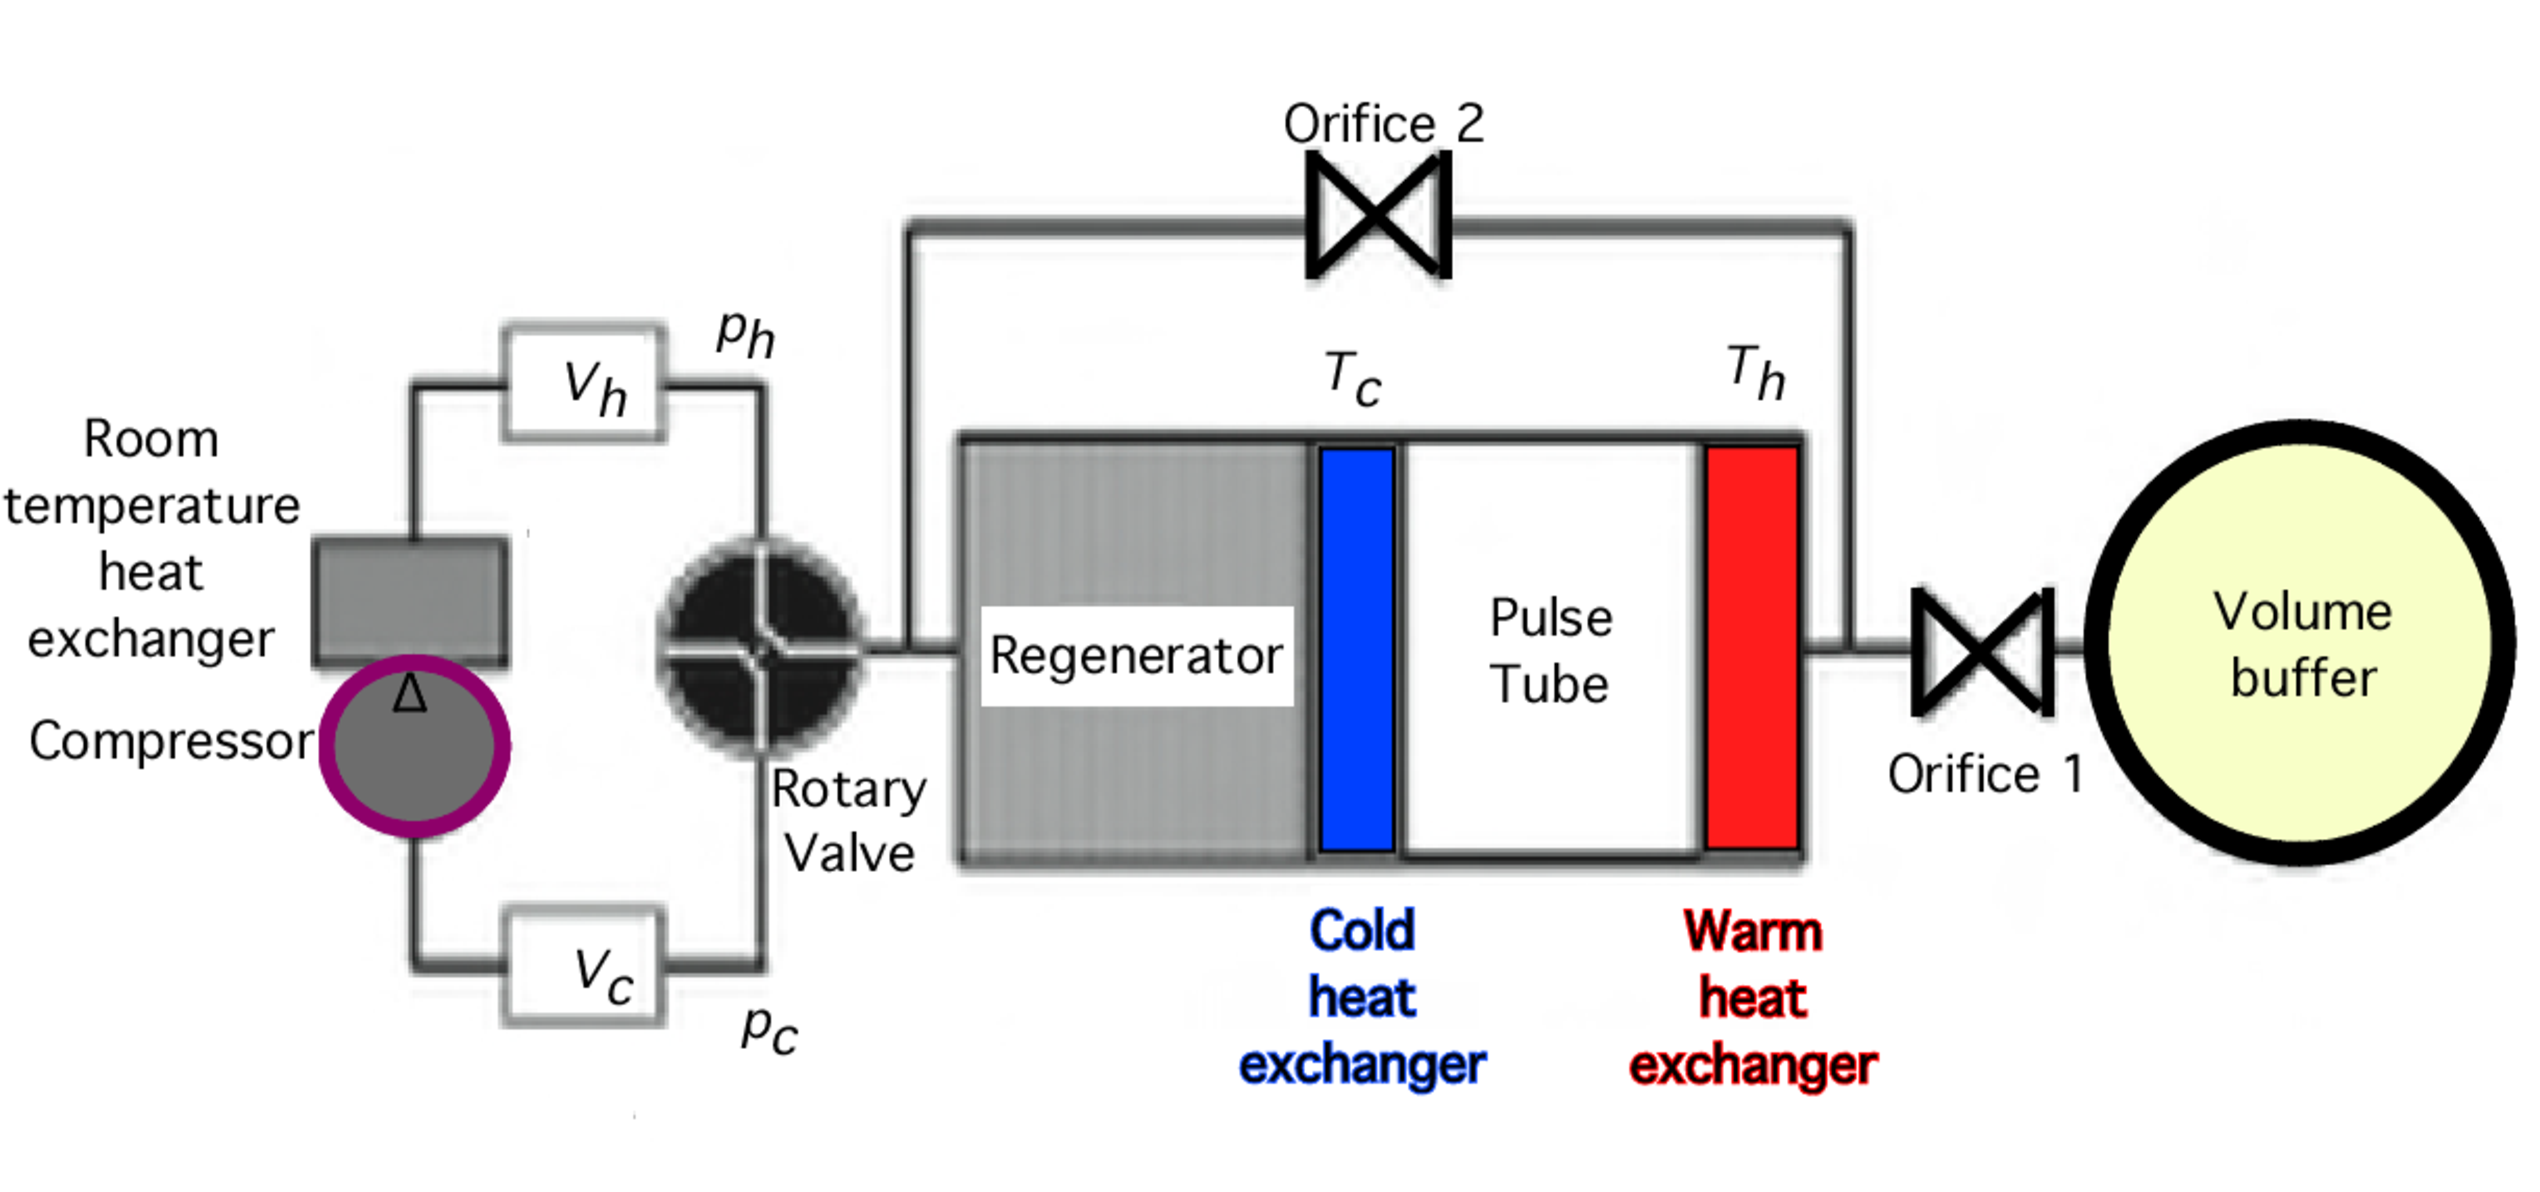
\includegraphics[width=10cm]{./Sec_SiteInfra/Figures/PT_scheme.pdf}
		\caption{Scheme of a Pulse Tube cryocooler.}
		\label{fig:cryo_infrastructure_figure/PT_scheme}
	\end{center}
\end{figure}
Let us consider a gas element entering the tube with temperature $T_h$ and leaving it with a higher temperature when the pressure in the tube is low.   Later in the cycle the same element is pushed out the tube again when the pressure inside the tube is high. As a consequence its temperature will be higher than $T_h$ . In the heat exchanger  it releases heat and cools to the ambient temperature $T_h$.
At the cold end of the pulse tube there is the opposite effect: here gas elements enter the tube  when the pressure is high with temperature $T_c$ and return when the pressure is low with a temperature below $T_c$. The heat is extracted from the cold point providing the desired cooling power.\\
The thermal environment of a gas element, that moves back and forth in the system, changes when it passes the heat exchanger. In the regenerator and in the heat exchanger the heat contact between the gas and its surrounding material is good. Here the temperature of the gas is practically the same as of the surrounding medium. However, in the pulse tube the gas element is thermally isolated, so, in the pulse tube, the temperature of the gas element varies with the pressure.\\
In 1984 Mikulin and his co-workers \cite{Mikulin} inserted a flow resistance (the orifice)  at the warm end of the pulse tube to allow some gas to pass to a large reservoir acting as buffer volume. This is typically 10 times larger than the volume of the pulse tube and its pressure is almost constant and close to the average pressure in the pulse tube. The combination of the orifice and the buffer provides a phase difference between the flow of the gas in the tube and the pressure oscillation; such phase difference is necessary for the performance of the PT.\\
In 1990, Zhu et al. \cite{Zhu} connected the warm end of the pulse tube with the main gas inlet by a tube, containing a second orifice. Thus, a part of the gas could enter the pulse tube from the warm end, bypassing the regenerator. The function of the second orifice  is to reduce losses. It allows some gas to bypass the regenerator and to enter the pulse tube directly.\\
The quality of the regenerator material set in practice the cryo cooler performance. It consists of a porous matrix of finely divided material in the form of wire mesh, plates or small balls. This form  maximizes the surface area and minimize the thermal conduction necessary within the solid to maximize the heat transfer with the surrounding gas within the duration of a cooling cycle. The regenerator stores the heat of the gas during a half-cycle and, therefore, it must have a high heat capacity, compared to the heat capacity of the gas.\\
At temperatures above $10$ K  materials as bronze or stainless steel  are often used.  Below $10$ K one uses rare earth materials, which are specially developed for this application.\\
To obtain temperatures below 20 K, the system is  operated at low frequency ( $\sim 1$ Hz ).
The frequency defines the diffusion depth $\delta$ in the working gas and the regenerator material:
$$d = \sqrt{\frac {k}{\pi \nu C}}$$
\noindent
where $k$ is the heat conductivity, $\nu$ is the frequency and $C$ is the volumetric heat capacity of the regenerator material. Thus, it follows that when the frequency is increased, the diffusion depth decreases, and the heat storage in the regenerator degrades.
Moreover, a high operating frequency leans to a large pressure drop in the regenerator, i.e.\ a poor performance of a system.}



Bibliografy

\bibitem { Mikulin}

\bibitem{Zhu}

=======================
FloatBarrier
\etbox{h}{box:information}{The Pulse Tube cryocooler} {The Pulse Tube cryocooler (PT) is based on the displacement and the expansion of a gas, usually helium (He$^4$).  A piston compressor and a rotary valve  are used to create the pressure oscillations ( the typical average pressure in a PT is $25}$ bar, and the oscillation amplitude is ranging between $2$ and  $7$ bar). Let us refer to the figure \ref{fig:PT_scheme} for explaining the thermal process.
\begin{figure}[H]
	\begin{center}
		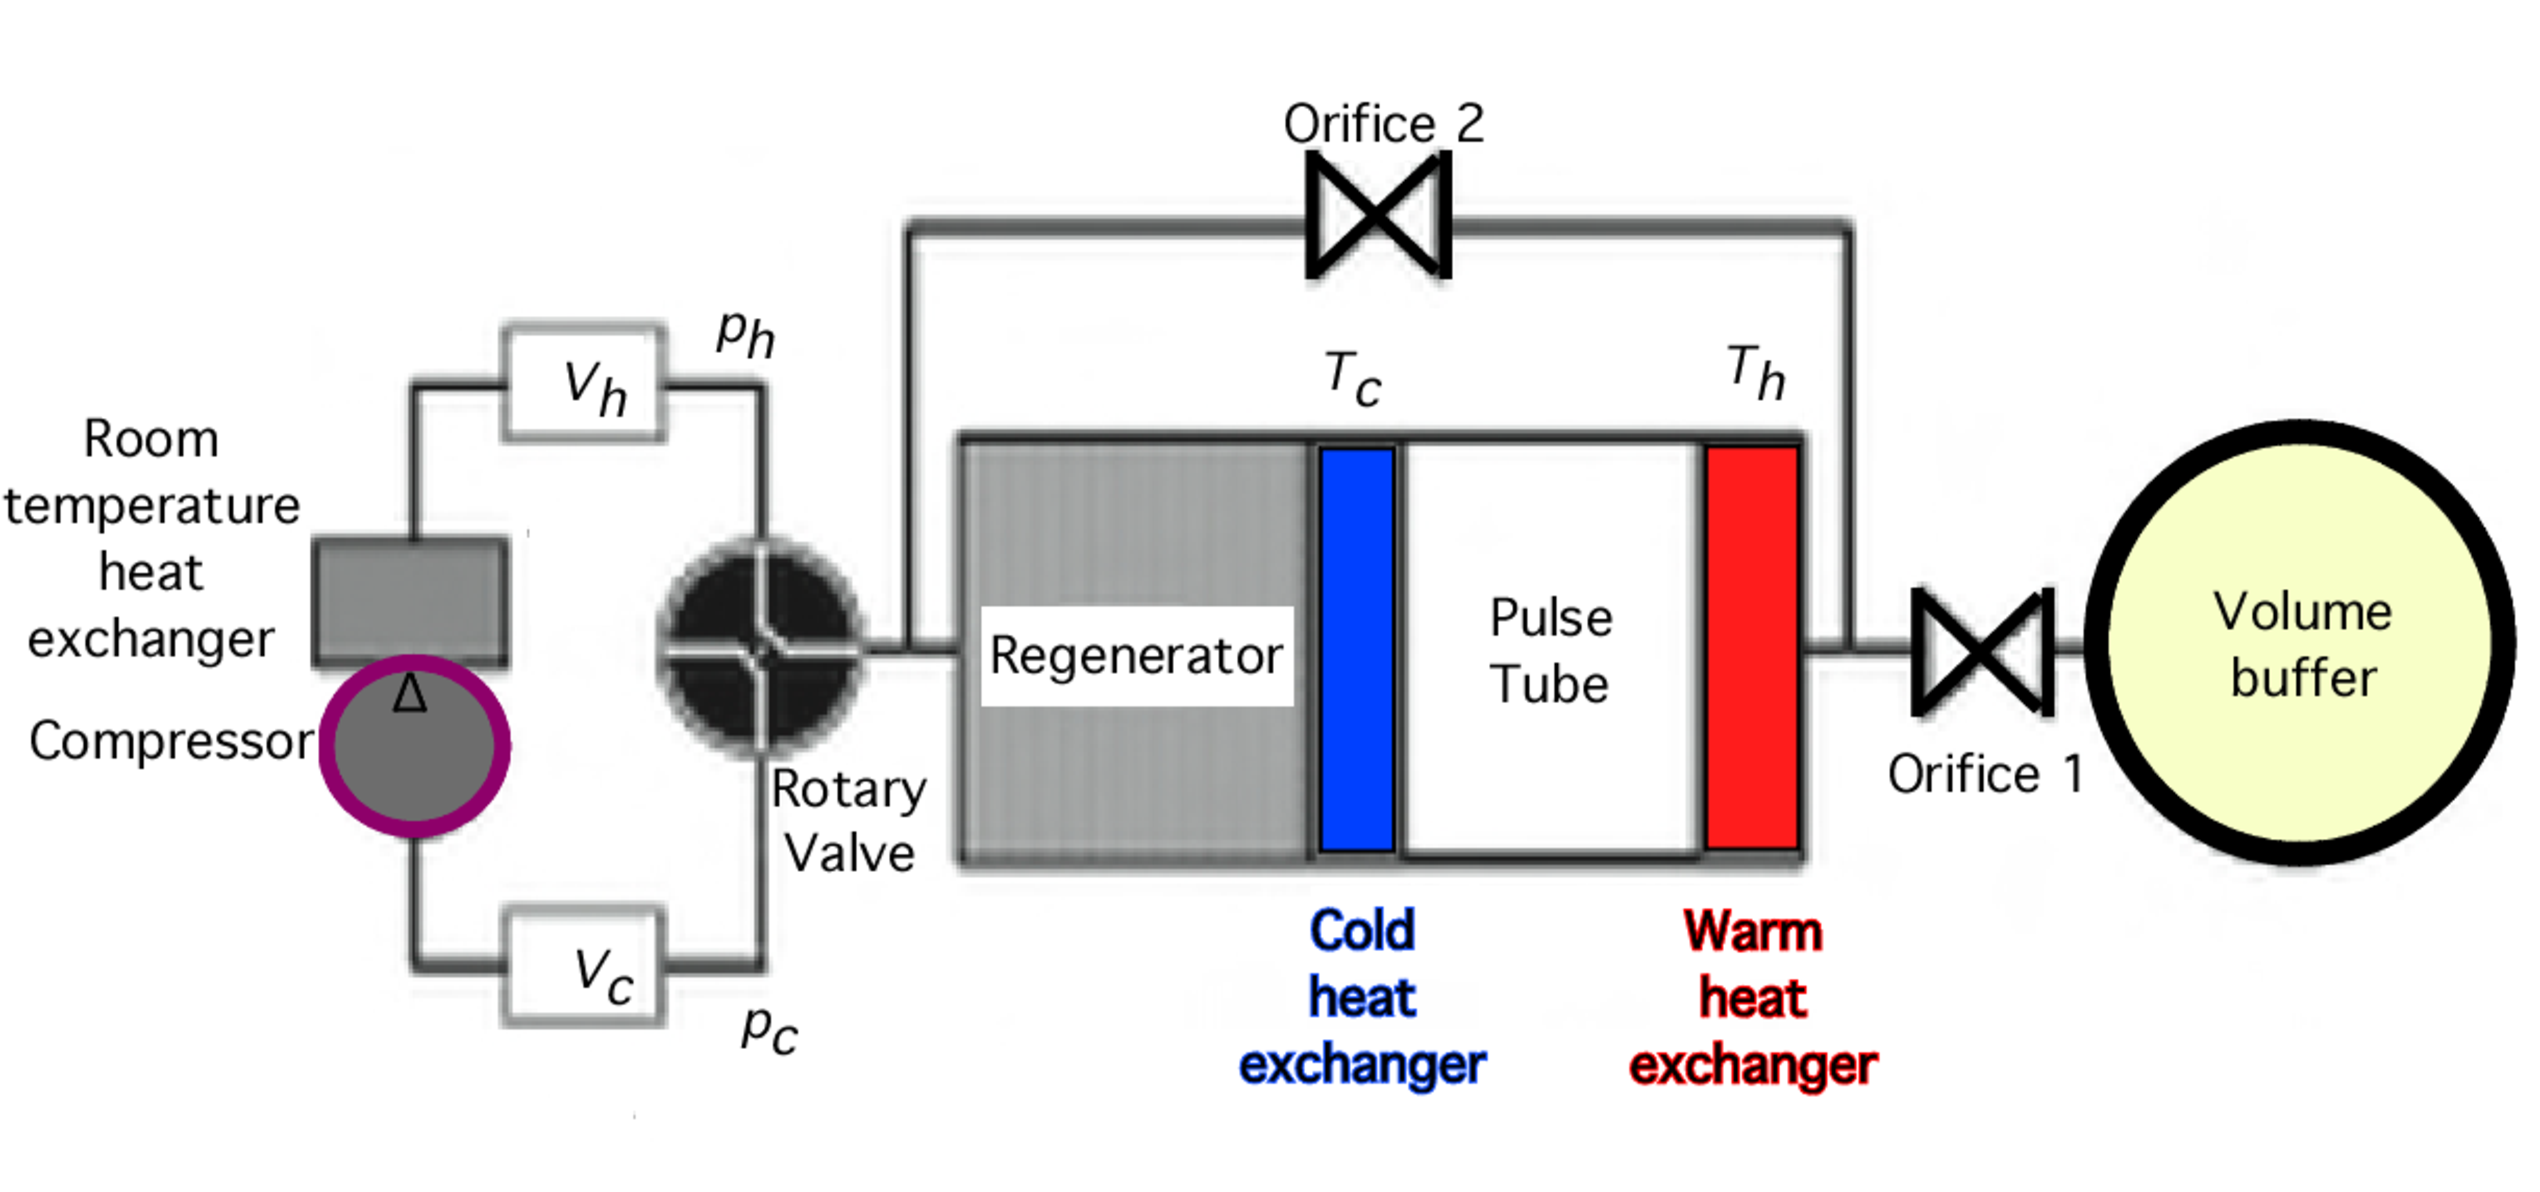
\includegraphics[width=9.5cm]{./Sec_SiteInfra/Figures/PT_scheme.pdf}
		\caption{Scheme of a Pulse Tube cryocooler.}
		\label{fig:PT_scheme}
	\end{center}
\end{figure}
We note that  a crucial element of the cryocooler is the  PT regenerator,  a heat exchanger acting as {\it cold storage} systems for the  pulsed flow process.   In practice, the regenerator  stores the energy from one stream and later transfer the energy to a second stream, for example between the out-of-phase pulses of gas. \\
The orifice 1  is connecting  the warm end  to a buffer volume, ten times larger than the volume of the pulse tube so that its pressure is almost constant and close to the average pressure in the pulse tube. The combination of the orifice and the buffer provides a phase difference between the flow of the gas in the tube and the pressure oscillation; such phase difference is necessary for optimizing the PT performance \cite{Mikulin}. The function of the second orifice  is to reduce losses allowing some gas to bypass the regenerator \cite{Zhu} .
\begin{itemize}
\item{When the pressure rises, the gas element moves through the regenerator in the direction of the cold heat exchanger. At the regenerator output  the temperature of the gas element is $T_c$ and enters the tube. There, the gas element is compressed adiabatically, while it moves towards the orifice and  Its temperature rises together with the pressure.}
\item{Now, the orifice 1 is open and  the gas  at pressure $p_h$ flows from the tube to the buffer since  the buffer pressure is lower than that of the tube.}
\item{ The orifice 1 is closed and the rotary valve is set to connect the system to the low-pressure side of the compressor ($p_c$). The gas moves back to the cold heat exchanger and the expansion takes place.  At the end of the expansion step, the pressure of the gas element is equal to $p_c$  and theits temperature is below $T_c$.}
\item{The expansion stops, and the orifice is open again. The gas continues to flow in the direction of  cold heat exchanger and when it is crossing it , the gas warms up to the temperature $T_c$. The amount of heat, which the gas takes away from the heat exchanger, is the cooling power.}
\end{itemize}
To obtain temperatures below 20 K, the system is  operated at low frequency ( $\sim 1$ Hz ).
The frequency defines the diffusion depth $\delta$ in the working gas and the regenerator material:
$$d = \sqrt{\frac {k}{\pi \nu C}}$$
\noindent where $k$ is the heat conductivity, $\nu$ is the frequency and $C$ is the volumetric heat capacity of the regenerator material. Thus, it follows that when the frequency is increased, the diffusion depth decreases, and the heat storage in the regenerator degrades.
Moreover, a high operating frequency leans to a large pressure drop in the regenerator, i.e.\ a poor performance of a system.}
\FloatBarrier